\documentclass[acmlarge,screen,natbib=false]{acmart}

% Font style CMR
\usepackage[T1]{fontenc}
\usepackage{lmodern}

% Algorithm
\usepackage{algorithm,algpseudocode}
\renewcommand\thealgorithm{\arabic{algorithm}:}

% Bibliography
\usepackage[backend=bibtex]{biblatex}
\addbibresource{ref.bib}

\usepackage{enumerate}

% ========== SOMETHING IMPORTANT ==========
\settopmatter{printacmref=false}
\renewcommand\footnotetextcopyrightpermission[1]{}
\pagestyle{plain}
\pagenumbering{gobble}
\def\BibTeX{{\rm B\kern-.05em{\sc i\kern-.025em b}\kern-.08emT\kern-.1667em\lower.7ex\hbox{E}\kern-.125emX}}

\begin{document}

%========== TITLE ==========
\title{Randomly Wired Recurrent Neural Networks}
\subtitle{Supervisors: Prof. Dr. Michael Granitzer, Julian Stier (Department of Computer Science, University of Passau)}

%========== AUTHOR ==========
\author{Darji, Harshil Jagadishbhai}

\makeatletter
\let\@authorsaddresses\@empty
\makeatother

%========= ABSTRACT ==========
\begin{abstract}
E-mail: darji01@ads.uni-passau.de\\
Matriculation: 87647
\vspace*{-2.4mm}
\end{abstract}

% ========== SOMETHING IMPORTANT ==========
\fancyfoot{}
\maketitle
\thispagestyle{empty}
\noindent\rule{12cm}{0.4pt}

% ========== INTRODUCTION ==========
\section{Introduction}
Recurrent Neural Networks (RNNs) are conventional models that have shown exceptional commitment in many NLP tasks that make use of sequential information. In traditional neural networks, it is assumed that all inputs are independent of each other, which is not a good idea for sequential tasks. For example, to predict the next word in a sentence, it is good to know words came before it. An RNN represents a sequence with a high-dimensional vector (called the hidden state) of a fixed dimensionality that incorporates new observations using an intricate nonlinear function \cite{is-phd-thesis}. In simple words, RNNs have a "memory" which captures knowledge about what has been calculated so far.

\begin{figure}[h!]
  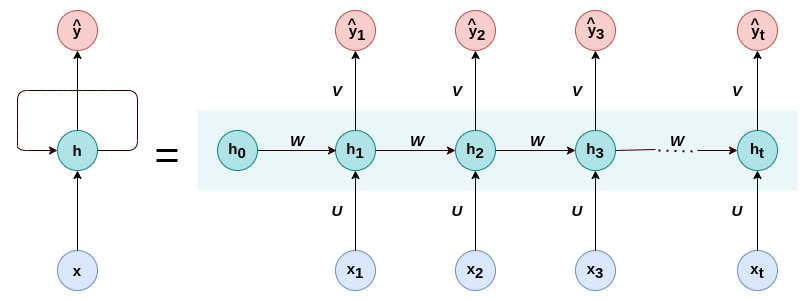
\includegraphics[scale=0.5]{rnn.png}
  \caption{A Recurrent Neural Network unfolded in time \cite{is-phd-thesis}}
  \label{fig:rnn}
\end{figure}

A standard RNN is parameterized with three weight metrices and three bias vectors [$W_{hv}, W_{hh}, W_{oh}, b_{h}, b_{o}, h_{o}$] whose concatenation $\theta$ fully descirbes the RNN (Fig. \ref{fig:rnn}). The RNN computes $h_{t}$ (sequence of hidden states) and $z_{t}$ (a sequence of outputs) by the following algorithm:

\begin{algorithm}
  \caption{A standard RNN algorithm \cite{is-phd-thesis}}\label{std_rnn}
  \begin{algorithmic}[1]
    \For{$t$ \textbf{from} $1$ \textbf{to} $T$}
        \State {$u_{t} \gets W_{hv}v_{t} + W_{hh}h_{t-1} + b_{h}$}
        \State {$h_{t} \gets e$($u_{t}$)}
        \State {$o_{t} \gets W_{oh}h_{t} + b_{o}$}
        \State {$z_{t} \gets g$($o_{t}$)}
    \EndFor
  \end{algorithmic}
\end{algorithm}
where $e$($\cdot$) and $g$($\cdot$) are the hidden and output nonlinearities of the RNN.

Deep extensions of such basic RNNs can be constructed by stacking multiple recurrent hidden states on top of each other as shown in \cite{drnn-2013}.

This thesis project aims to produce randomly wired deep RNN architectures by embedding random graph models in-between the input and output layer and then introducing a recurrent connection to make them dependent on early sequences.

% ========== MOTIVATION ==========
\section{Motivation}
In April 2019, Researchers from the Facebook AI Research group published a paper \cite{randnn} in which they explored randomly wired neural networks driven by random graph models from graph theory. Authors claim that the mean accuracy of these models is competitive with hand-designed and optimized models from recent works on neural architecture search. This approach successfully shows that even randomly wired networks have an exceptional performance on image classification. If a similar approach is applied to Recurrent Neural Networks, there is a chance that these randomly wired networks will provide results better or comparable to existing hand-designed models.

In September 2019, researchers from the University of Passau published a paper \cite{julian} in which they tried to predict the performance of convolutional neural networks before actually training them. To achieve this, they first used random graph generators to generate graphs with desired properties. Then the next step was to make them directed and to compute layer indexing of all vertices. Then they embed layered vertices between an input and output layer of an Artificial Neural Network that meets the requirements of the dataset. The authors created a dataset of such 10000 graphs and split it into a train-test with a 70-30 ratio. They trained neural architectures of train sets and stored their performances along with their graph properties. Then they used this data to train three different learning algorithms and used them to estimate model performance values of architectures of the test set using their underlying structural properties. This paper provides motivation to predict the performance of RNNs based on their internal structural properties which will be really helpful given the fact that it is always difficult to train RNNs due to its exploding/vanishing gradients.

% ========== RESEARCH QUESTIONS ==========
\section{Research goals}
Sparsity and randomness in recurrent neural networks are still not explored much compared to CNNs. Therefore, the main focus of thesis is to:
\begin{enumerate}[	1.]
	\item Explore and explain sparsity in Recurrent Neural Networks
	\item Investigate how the sparse and random architectures affect the performance of RNNs
\end{enumerate}

% ========== EXPERIMENT(S) ==========
\section{Experiments}
To investigate the effects of sparsity on the performance of RNNs, two of the experiments, to begin with, is described as follow:
\begin{enumerate}[	1.]
	\item Investigating the performance of pruned RNNs:
	\begin{enumerate}[-]
		\item Train RNNs repeatedly for certain epochs,
		\item Retrieve the weight distribution for hidden-to-hidden matrices,
		\item Prune weights below a certain threshold and analyze its effect on the overall performance,
		\item Investigate the performance of pruned RNN in comparison with standard RNN and its different variations (e.g. LSTM, GRU).
	\end{enumerate}
	\item Investigating the performance of sparse RNNs:
	\begin{enumerate}[-]
		\item Construct sparse RNN architecture (as described in \S\ref{construct_sparse_rnn}),
		\item Train sparse RNNs repeatedly for certain epochs,
		\item Compare performance of sparse RNN with pruned RNN, standard RNN and its different variations.
	\end{enumerate}
\end{enumerate}

% ========== METHODOLOGY ==========
\section{Construction of sparse RNN} \label{construct_sparse_rnn}
To create randomly wired sparse RNN, the methodology followed is influenced by the process introduced in \cite{julian} and \cite{randnn}.
\begin{enumerate}[	1.]
	\item The first step is to generate random graphs without restricting how the graphs correspond to neural networks (Fig. \ref{fig:rgg}).
	\item Once the graph is generated, it is necessary to make it directed where edges define the data flow (Fig. \ref{fig:dag}).
	\item The next step is to compute layer indexing of all vertices of the available Directed Acyclic Graph (DAG).
	\item By embedding these layered vertices between an input and output layer completes the structure of a sparse neural network (Fig. \ref{fig:layered_arch}).
	\begin{figure}[h!]
		\minipage{0.32\textwidth}
			\begin{center}
				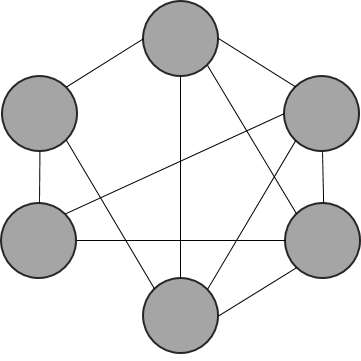
\includegraphics[scale=0.5]{rgg.png}
			\end{center}
  			\caption{Randomly generated graph \cite{julian}}
  			\label{fig:rgg}
		\endminipage\hfill
		\minipage{0.32\textwidth}
			\begin{center}
 				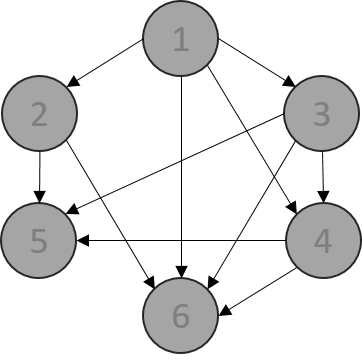
\includegraphics[scale=0.5]{dag.png}
			\end{center}
  			\caption{Transformed DAG \cite{julian}}
  			\label{fig:dag}
		\endminipage\hfill
		\minipage{0.32\textwidth}
			\begin{center}
  				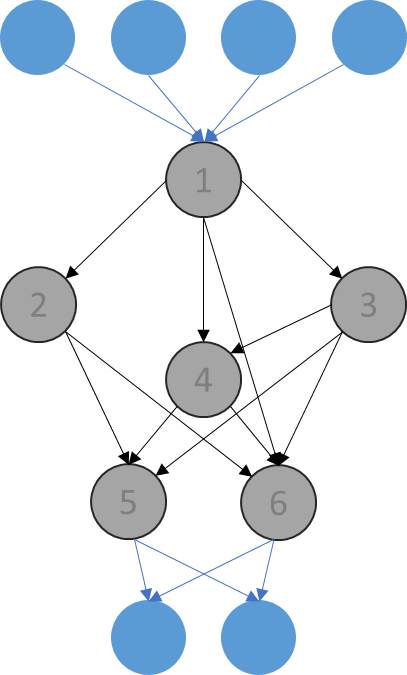
\includegraphics[scale=0.5]{layered_arch.png}
			\end{center}
  			\caption{Embedded DAG after computing layered indexing \cite{julian}}
  			\label{fig:layered_arch}
		\endminipage
	\end{figure}
	\item This generated structure is a simple feed-forward network, as defined in \cite{julian}. To convert it into a recurrent architecture, it is necessary to introduce recurrent connections that make subsequent runs dependent on previous runs (Fig. \ref{fig:randwirernn}).
	\begin{figure}[h!]
  		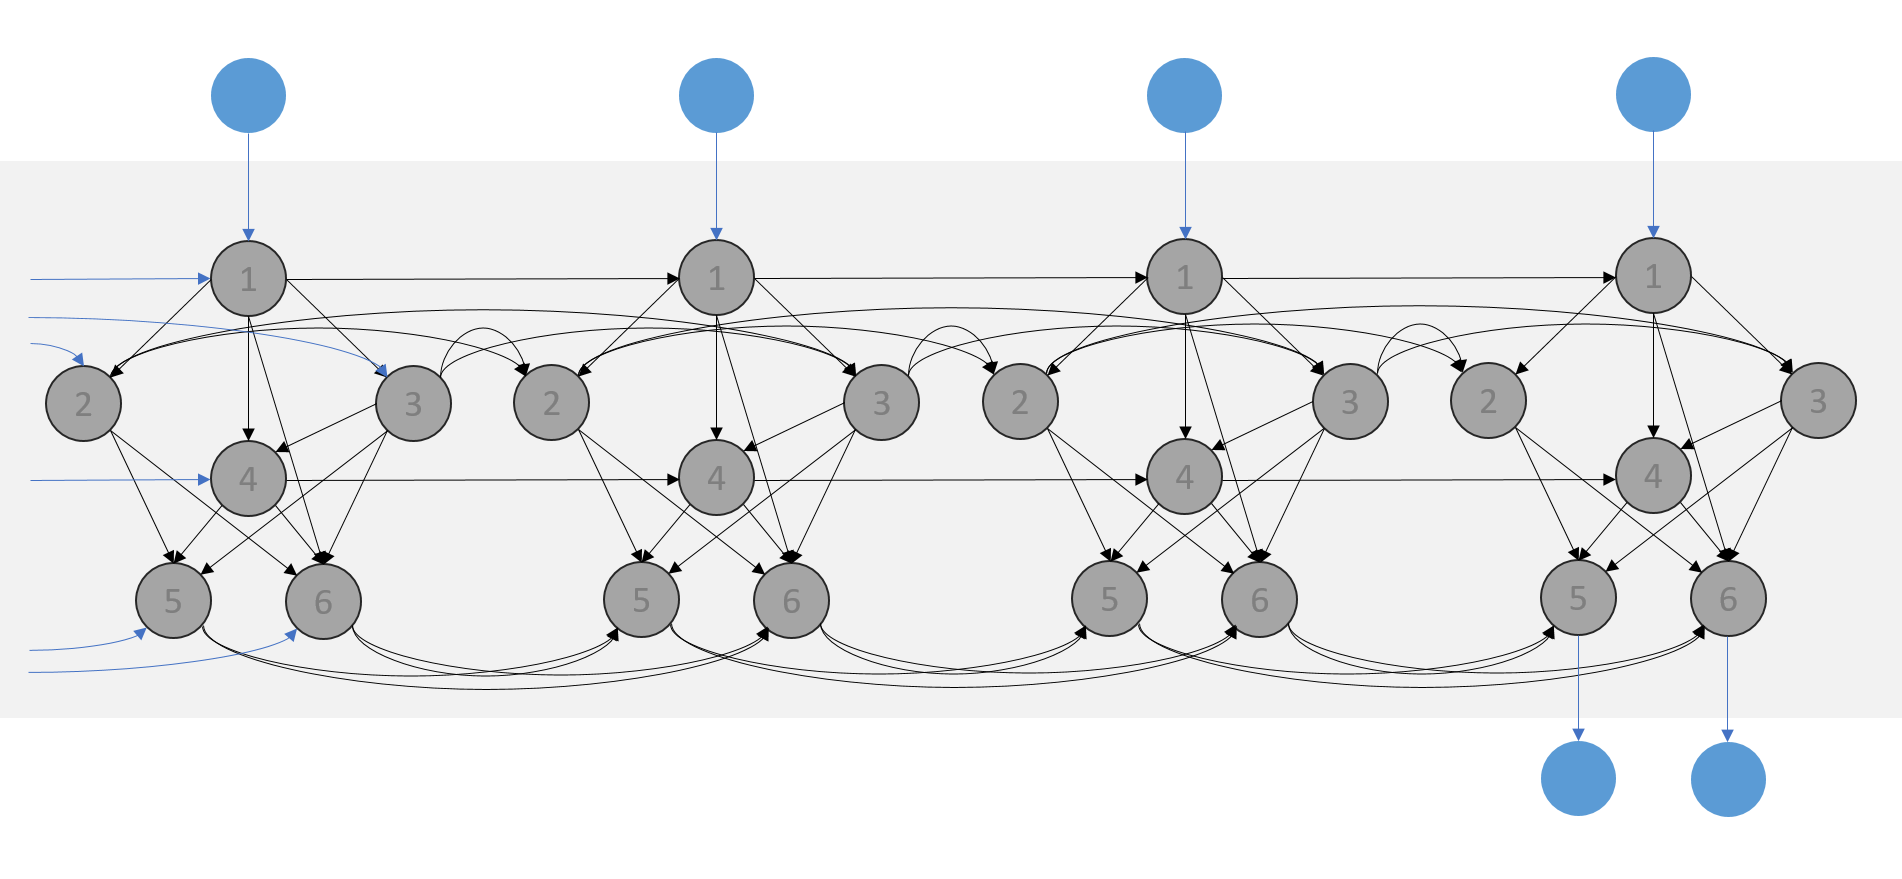
\includegraphics[scale=0.5]{RandWiredRNN.png}
  		\caption{Above generated feed-forward (Fig. \ref{fig:layered_arch}) transformed into RNN and opened in-time.}
  		\label{fig:randwirernn}
	\end{figure}
	\item Once the complete structure is available, it will be trained on the training set and then will be evaluated on the test set.
\end{enumerate}


% ========== DATASET ==========
\section{Dataset}
The choice of the dataset depends on the type of RNN being implemented.
\begin{enumerate}[	1.]
	\item \textbf{Many-to-One: }This type of RNNs is mainly used for the classification task such as Twitter or IMDB sentiment analysis. Therefore, examples of the datasets can be used are (un)labeled Twitter/IMDB dataset, Reber grammar dataset, etc.
	\item \textbf{One-to-Many: }This type of RNNs is mainly used for sequence generation tasks such as generating texts or grammar strings. Example datasets are Shakespeare's text, Show scripts, Reber grammar, etc.
\end{enumerate}
As can be seen, the Reber grammar dataset can be used for classification as well as sequence generation tasks. Therefore, in the beginning, to check the pipeline, the Reber grammar dataset will be used. Once the stable implementation is available, the implementation will be tweaked to make it flexible to work with any other datasets.

% ========== EVALUATION ==========
\section{Evaluation}
Although it is known that accuracy cannot be considered as an impeccable evaluation technique, this project aims at using accuracy to justify the performance of sparse and randomly wired recurrent neural networks. As stated before, one of the main focuses of the thesis is to investigate the effects of sparsity and randomness of RNNs on its performance, accuracy can be considered as a simple and effective way to compare results.

% ========== SCHEDULE ==========
\section{Schedule}
The schedule is divided into four major tasks i.e, research, implementation, evaluation and documentation. The following table gives information about the amount of time required to finish each task.
\begin{table}[H]
\begin{tabular}{cc}
	\toprule
	Task & Duration (weeks)\\
	\midrule
	Research & 4\\
	Implementation & 10\\
	Testing & 2\\
	Documentation & 8\\
	\bottomrule
\end{tabular}
\caption{Schedule of the thesis}
\end{table}


% ========== REFERENCES ==========
\printbibliography

\end{document}
